\documentclass[oneside,final,14pt]{extreport}

%% my command
%%%%%%%%%%%%%%
% Путь к файлу с изображениями
\newcommand{\picPath}{pictures}
% Величина отступа
\newcommand{\indentSpace}{1.25cm}
% Сокращения
\newcommand{\urlTitle}{ $-$ URL: }
%%%%%%%%%%%%%%%


% Изменяем шрифт
\usepackage{fontspec}
\setmainfont{Times New Roman}
\listfiles

% Полуторный интервал
\linespread{1.6}

% Отступ
\setlength\parindent{\indentSpace}

% Математика
\usepackage{mathtools}


% Картинки
\usepackage{graphicx}
\usepackage{subcaption}

% Языковой пакет
\usepackage[russianb]{babel}

% Таблицы
\usepackage{tabularx}

% Настройка подписей к фигурам
% Меняем заголовки картинок
\usepackage[ labelsep= endash]{caption}
\captionsetup{%
   figurename= Рисунок,
   tablename= Таблица,
   justification= centering% Формат - по центру
}         

% Кирилица в подфигурах
\renewcommand{\thesubfigure}{\asbuk{subfigure}}
% разделитель в подфигурах - правая скобка
\DeclareCaptionLabelSeparator{r_paranthesis}{)\quad }
\captionsetup[subfigure]{labelformat=simple, labelsep=r_paranthesis}

% Добавляем итератор \asbuk,
% чтобы использовать кирилицу
% как маркеры
\usepackage{enumitem}
\makeatletter
\AddEnumerateCounter{\asbuk}{\russian@alph}{щ}
\makeatother

% Меняем маркеры в перечислениях
% Списки уровня 1
\setlist[enumerate,1]{label=\arabic*),ref=\arabic*}
% Списки уровня 2
\setlist[enumerate,2]{label=\asbuk*),ref=\asbuk*}
% Перечисления
\setlist[itemize,1]{label=$-$}
% Удаляем отступы перед и после
% списка
\setlist[itemize]{noitemsep, topsep=0pt}
\setlist[enumerate]{noitemsep, topsep=0pt}

% Красная строка в начале главы
\usepackage{indentfirst}

% Убиваем перенос
\usepackage[none]{hyphenat}

% Перенос длинных ссылок
\usepackage[hyphens]{url}
\urlstyle{same}

% Выравнивание по ширине
\usepackage{microtype}

% Косая черта в таблице
\usepackage{diagbox}
\usepackage{makecell}

% Границы
\usepackage{vmargin}
\setpapersize{A4}
% отступы
%\setmarginsrb 
%{3cm} % левый
%{2cm} % верхний
%{1cm} % Правый
%{2cm} % Нижний
%{0pt}{0mm} % Высота - отступ верхнего колонтитула
%{0pt}{0mm} % Высота - отступ нижнего  колонтитула

\setlength\hoffset{0cm}
\setlength\voffset{0cm}
\usepackage[top=2cm, bottom=2cm, left=3cm, right=2cm,
]{geometry}
 		
% Настройка заглавиий
\addto\captionsrussian{% Replace "english" with the language you use
  \renewcommand{\contentsname}% содержания
    {\hfill\bfseries
    СОДЕРЖАНИЕ
	\hfill    
    }%
   \renewcommand{\bibname}% списка источников
    {\hfill\bfseries
    	СПИСОК ИСПОЛЬЗОВАННЫХ ИСТОЧНИКОВ
	\hfill
	}% 
}%\

%\renewcommand{\contentsname}{\hfill\bfseries СОДЕРЖАНИЕ \hfill} 

% Настройка  заглавий в главах
\usepackage{titlesec}


%\titleformat
%{\chapter} % command
%[display]
%{
%\bfseries
%} % format
%{
%\thechapter.
%} 	% label
%{ 
%	0 pt
%} % sep
%{    
%\centering
%} % before-code

\titleformat{\chapter}
            {\bfseries}
            {\hspace{\indentSpace}\thechapter\hspace{1em}}
            {0pt}
            {
            \vspace{0mm} }
            [\vspace{14pt}]% Отступ после
% Начальный сдвиг заголовка 50 pt = 1.763888888cm.
% Второй параметр- сдвиг до = 2cm - 50pt
\titlespacing{\chapter}{0pt}{-0.2361cm}{0pt}

\titleformat{\section}
{\bfseries}{\hspace{\indentSpace}\thesection}{1em}{}

%\titleformat{\section}
%            {\bfseries}
%            {\thechapter.\hspace{1em}}
%            {0pt}
%            {\centering
%            \vspace{0mm} }
%            [\vspace{14pt}]% Отступ после
%\titlespacing{\section}{0pt}{-50pt}{0pt}

% Конец настройка заглавий

% Форматирование списка источников
\makeatletter
\renewcommand*{\@biblabel}[1]{\hfill#1}
\makeatother

% Убрать отсупы в списке источников
\usepackage{lipsum}

% ADD THE FOLLOWING COUPLE LINES INTO YOUR PREAMBLE
\let\OLDthebibliography\thebibliography
\renewcommand\thebibliography[1]{
  \OLDthebibliography{#1}
  \setlength{\parskip}{0pt}
  \setlength{\itemsep}{0pt plus 0.3ex}
}



% Добавить точки в оглавление
\usepackage{tocstyle}
\newcommand{\autodot}{.}


% Чтобы картинки вставляись
% куда надо
\usepackage{float}

% Режим релиза
\sloppy
\usepackage{layout}

\begin{document}
%Статистический анализ текстовой информации вебинаров
%\newpage
\tableofcontents
\newpage
\begin{center}
\bfseries ВВЕДЕНИЕ
\end{center}
\addcontentsline{toc}{chapter}{Введение}

В Сибирском государственном университете телекоммуникаций и информатики,с которым у КубГУ имеется соглашение о сотрудничестве в сфере образования, науки, научной и инновационной деятельности стоит задача оценивания
качества контактной работы, реализуемой посредством вебинаров, в ходе дистанционного обучения. 

Для решения этой задачи разработана математическая модель, которая включает систему из 32 показателей качества организации и проведения вебинара (перечень которых представлен в приложении), позволяющих оценить с разных сторон  качество вебинара 10-балльными экспертными оценками. Проблема заключается в существенных трудозатратах, которые несут эксперты при оценивании этих показателей. Кроме того, мнения экспертов субъективны, а задача поставлена максимально объективизировать процедуру оценивания, например, за счет минимизации влияния человеческого фактора в процедуре оценивания. В связи с этим актуальной является  задача разработки такой компьютерной технологии, которая позволит оценить максимальное количество показателей без участия человека в автоматическом режиме. В числе показателей, которые могут быть автоматически при помощи некоторого алгоритма входят: колличество и качество информации на слайдах, использование указки, точность заявленной длительности мероприяти и тд.

Основой для анализа данных показателей является три основных аспекта:
\begin{itemize}
\item поиск указки;
\item выделение слайдов;
\item распознавание блоков текста на слайдах.
\end{itemize} 

Для решения вышеперечисленных задач в ходе курсовой работы проведен анализ следующих процедур над изображениями:

\begin{itemize}
\item поиск границ объектов;
\item поиск вхождения одного изображения в другое;
\item вычисление коэфициента схожести изображений;
\item локализация текста.
\end{itemize}

Программно разработаны процедуры, реализующие основу для дальнейшего развития приложения автоматического вычисления основных критериев оценки вебинаров. В реализации используется бесплатная библиотека машинного зрения OpenCV. 

\chapter{Методы определения границ объектов на изображении}
Границы объектов на изображении характеризуются изменением яркости в некотором направлении. Выделяют три вида границ: идеальные,  размытые  и крышевидные. На рисунке \ref{fig:contours}  изображены вертикальные границы трех видов.

\begin{figure}[H]
  \centering
  \begin{subfigure}[b]{0.4\linewidth}
    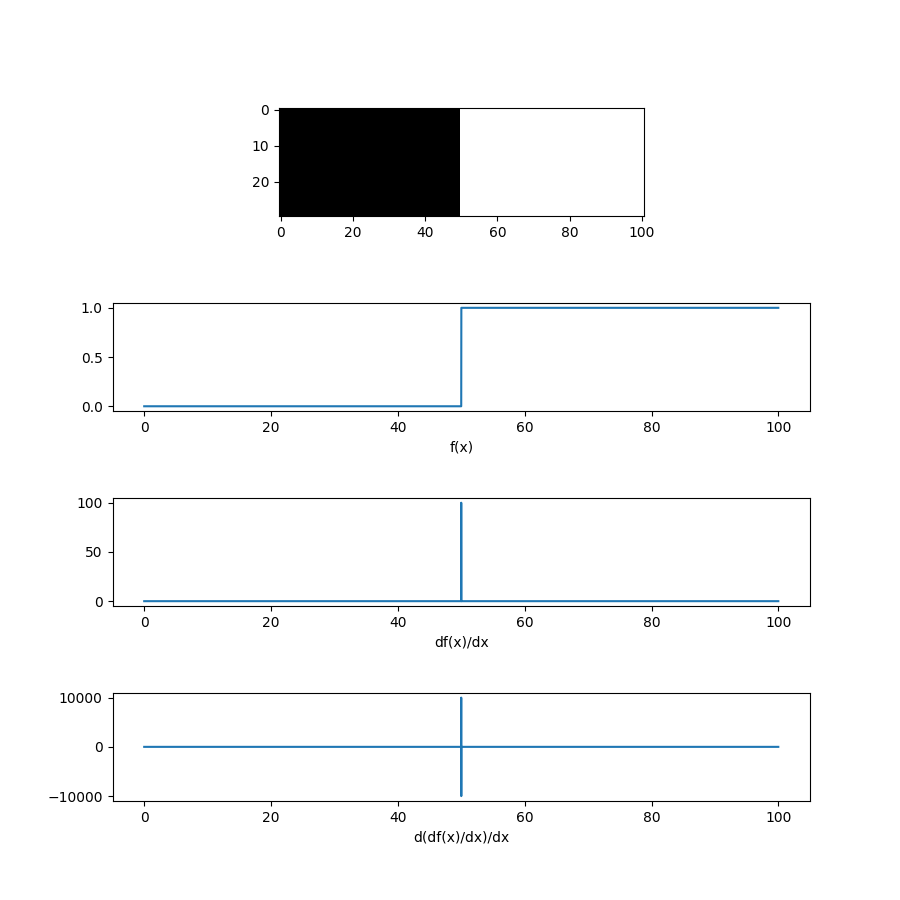
\includegraphics[width=\linewidth]{\picPath/perfect.png}
    \caption{ Идеальная граница}
  \end{subfigure}
  \begin{subfigure}[b]{0.4\linewidth}
    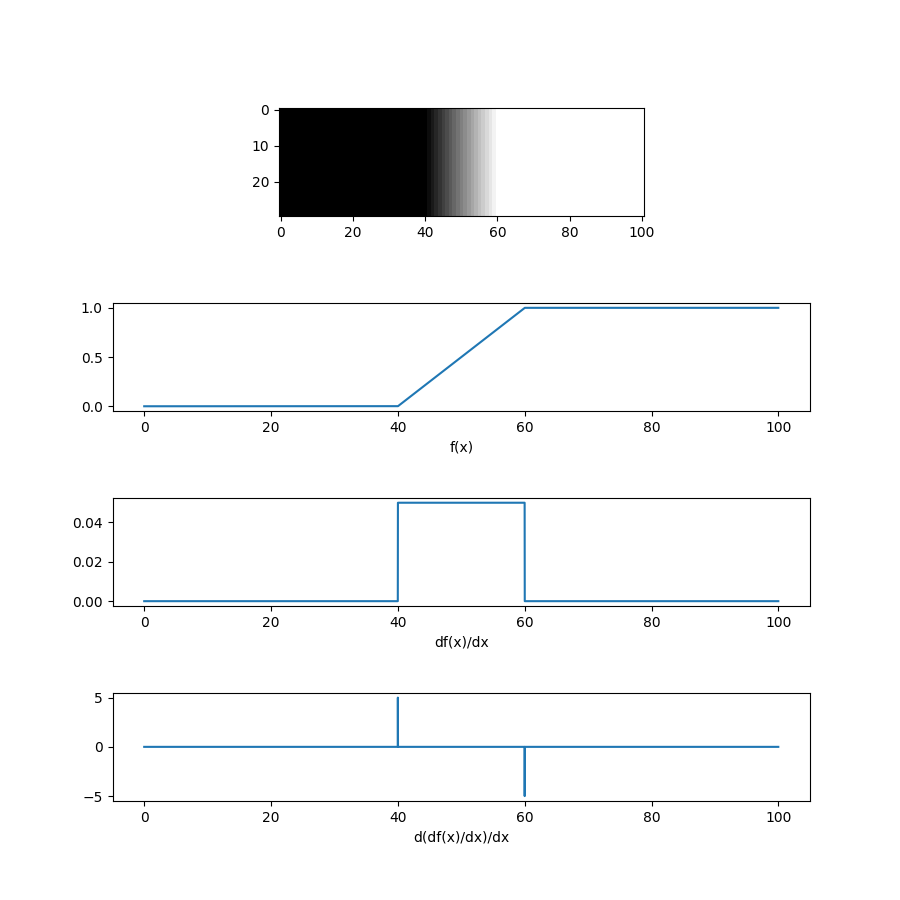
\includegraphics[width=\linewidth]{\picPath/smooth.png}
    \caption{Размытая граница}
  \end{subfigure}
  \begin{subfigure}[b]{0.4\linewidth}
    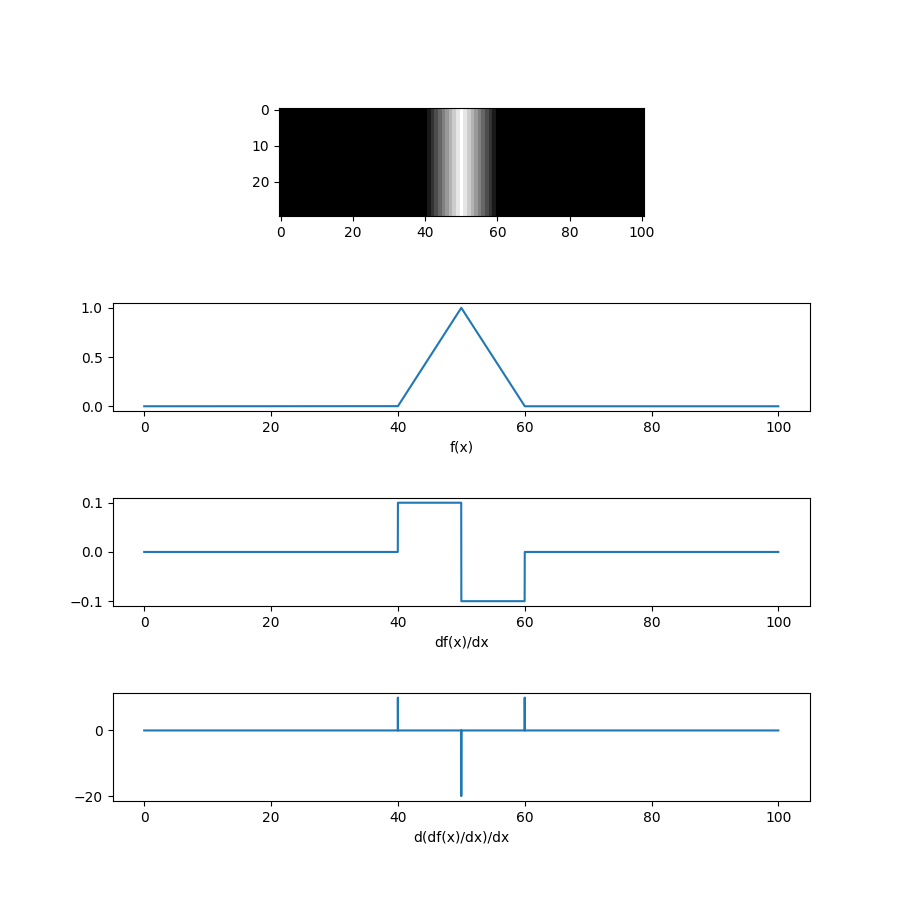
\includegraphics[width=\linewidth]{\picPath/roof.png}
    \caption{Крышевидная граница}
  \end{subfigure}
  \caption{границы объектов: изображение, функция яркости, первая и вторая производные}
  \label{fig:contours}
\end{figure}

Рассмотрим вертикальную размытую границу. Тогда зафиксировав ординату, получим дискретную функцию от одной переменной $g(x)$. Рассмотрим её первую и вторую производные: первая производная равна нулю в областях, где интенсивность постоянна и равна константе на границе, причем константа тем больше, чем уже граница. Вторая производная не равна нулю только в координатах начала и конца границы $g(x)$, в этих точках она равна бесконечности. Для случая крышевидной границы, первая производная положительна на подъеме и отрицательна на спуске границы. Вторая производная не ноль в трех точках, причем граница помещается между первой и последней не нулевой точкой второй производной. Отсюда следует вывод: зная направление границы, её координаты находятся из производной функции интенсивности по этому направлению. 
 
В общем случае, если заранее неизвестны направления границ объектов, за направление берут направление максимального роста интенсивности  то есть градиент изображения, если представлять его как дискретную функцию от двух переменных. 

Градиент есть вектор частных производных:
\begin{equation}
\nabla f(x,y) 
= 
grad[f(x,y)]
=
\begin{bmatrix}
g_x(x,y)\\
g_y(x,y)
\end{bmatrix}
=
\begin{bmatrix}
\frac{\partial f(x,y)}
{\partial x}\\
\frac{\partial f(x,y)}
{\partial y}
\end{bmatrix}
\end{equation}

 На практике производные вычисляются численно, разностными методами. Если принять расстояние между соседними в строке и соседними в столбце пикселями за единицу, компоненты градиента с точностью $O(1)$ вычисляется по формулам:

\begin{gather}
g_x(x,y) 
= 
\frac{\partial f(x,y)}
{\partial x}
=
f(x+1,y) - f(x,y)
\\
g_y(x,y) 
= 
\frac{\partial f(x,y)}
{\partial y}
=
f(x,y+1) - f(x,y)
\end{gather}

Что равносильно свертке изображения \cite{Dup:coursache} с ядрами 
\begin{equation}
\begin{bmatrix}
-1\\1
\end{bmatrix}
\quad
\begin{bmatrix}
-1 & 1
\end{bmatrix}
\end{equation}

На практике для вычисления градиента используются оператор Собеля:
\vspace{3mm}
\begin{equation}
\begin{bmatrix}
 -1 & \,2 & -1 \\
\,0 & \,0 &\,0 \\
\,1 & \,2 &\,1
\end{bmatrix}
\quad
\begin{bmatrix}
-1 & 0 &  1 \\
-2 & 0 &  2 \\
-1 & 0 &  1
\end{bmatrix}	
\end{equation}

\vspace{3mm}Конечное изображене вычисляется 	по формуле
\begin{equation}
G
=
|G_x| + |G_y|
\end{equation}

Где $G_x$ и $G_y$ - результат свертки изображения с первым и вторым ядром оператора Собеля соответсвенно.
 
В результате применения оператора Собеля на изображении белым цветом выделены предполагаемые границы. Градиентный метод Собеля выделения границ широко используется в прикладных задачах благодаря своей простоте и высокой точности. К недостаткам метода Собеля можно отнести зависимость от шумов: при достаточно высоком их содержании алгоритм не способен адекватно определить границы объектов.



\chapter{Методы сравнения изображений}
\section{Сравнение гистограмм}
Метод сравнения гистограмм - один из самых простых и быстрых способов сравнения  двух изображений. Алгоритм основан на предположении о том, что похожие изображения имеют похожие цвета. 

Гистограмма это график  или функция распределения элементов цифрового изображения с различной яркостью. Гистограмма определена на множестве всех возможных значений яркостей чёрно-белого изображения, значение функции равно количеству пикселей, яркость которых равна аргументу гистограммы. В общем случае значение яркости - $n$ мерный вектор. Обычно для сравнения цветных изображений используются каналы HS цветового пространства HSV. Это основано на том, что при сравнении цвета разной яркости не различают, а поэтому канал V, отвечающий за яркость цвета игнорируют.  

Для сравнения гистограмм в openCV используется одна из метрик. Сравнение работы алгоритма с разными метриками на тестовых рисунках \ref{hist:pics} представленно в таблице \ref{hist:comparison}.  

Correlation  CV\_COMP\_CORREL
 
$$
d(H_1,H_2) 
= 
\frac{
\sum_I(H_1(I) - \overline{H}_1)
(H_2(I)-\overline{H}_2)
}{
	\sqrt{
		\sum_I(H_1(I) - \overline{H}_1)^2
		\sum_I(H_2(I) - \overline{H}_2)^2
	}
}
$$
$$
\overline{H}_k 
= 
\frac{1}{N}
\sum_J H_k(J)
$$

Chi-Square ( CV\_COMP\_CHISQR )
$$
d(H_1,H_2)
=
\sum_I \frac{
	(H_1(I) - H_2(I))^2}
{H_1(I)}
$$

Intersection ( method=CV\_COMP\_INTERSECT )

$$
d(H_1,H_2)
=
\sum_I 
\min (H_1(I),H_2(I))
$$

Bhattacharyya distance ( CV\_COMP\_BHATTACHARYYA )
$$
d(H_1,H_2)
=
\sqrt{ 1 - 
\frac{1}{
  \sqrt{\overline{H}_1 
  		\overline{H}_2
  		N^2}
  }
  \sum_I
  \sqrt{H_1(I) H_2(I)}
}
$$

Где $I$ в общем случае вектор, сумма идет по всем возможным векторам.


Достоинства данного метода - инвариантность относительно формы и размера сравниваемых изображений.

Главный недостаток метода сравнения гистограмм -   разделение изображений весьма условно. Каждому изображению подобно всё множество изображений, составленных из тех же пикселей, расположенных в произвольном порядке. Поэтому данный метод не подходит, например,  для задачи поиска курсора так как существует вероятность того, что на изображении, кроме курсора, могут находиться элементы, гистограммы которых очень близки к гистограмме курсора.   

\begin{figure}[H]
\begin{center}
\begin{subfigure}[b]{0.2\linewidth}
    	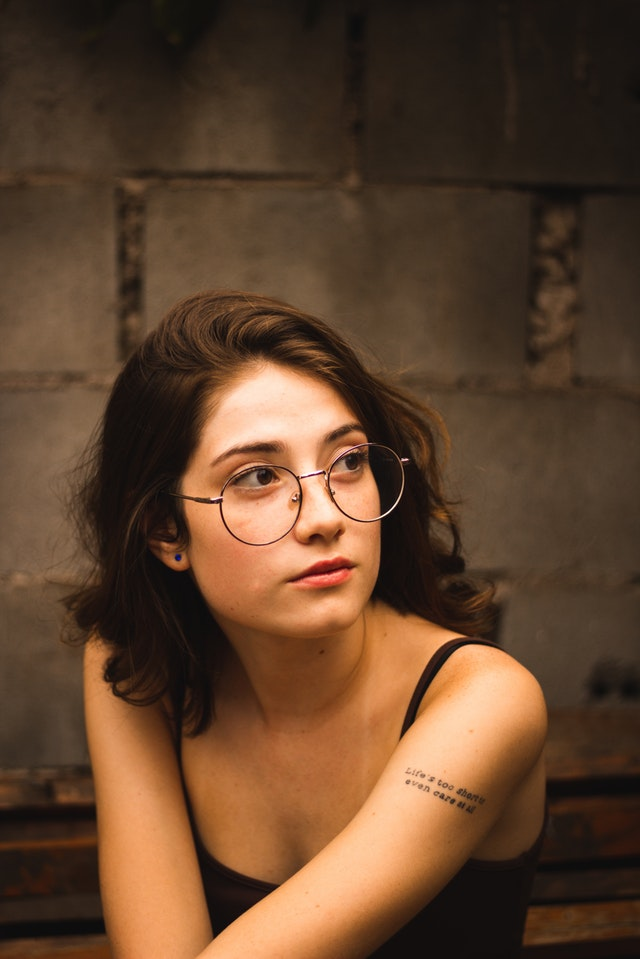
\includegraphics[width=\linewidth]{\picPath/girl.jpg}
    	\caption{ girl.jpg}
  \end{subfigure}
  \begin{subfigure}[b]{0.3\linewidth}
    	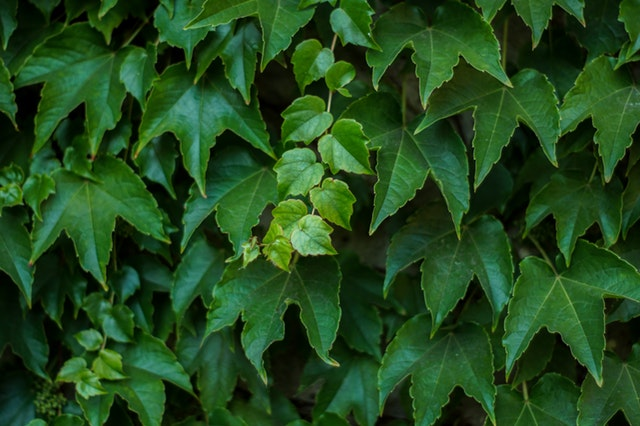
\includegraphics[width=\linewidth]{\picPath/leafs.jpg}
    	\caption{ leafs.jpg}
  \end{subfigure}
  \begin{subfigure}[b]{0.3\linewidth}
    	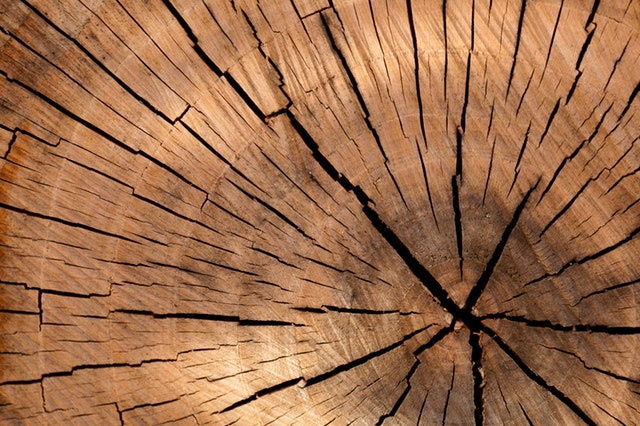
\includegraphics[width=\linewidth]{\picPath/wood.jpg}
    	\caption{ wood.jpg}
  \end{subfigure}
\end{center}
  \caption{изображения, используемые в сравнительном тесте  }
  \label{hist:pics}
\end{figure}

\begin{table}[H] 
\caption{cравнение результатов сравнения изображений по гистограмме}
\label{hist:comparison}
\begin{tabularx}{\textwidth}{|X|X|X|X|X|}
\hline
 & 
girl.jpg сравнить с girl.jpg
&
girl.jpg сравнить с leafs.jpg
&
girl.jpg сравнить с wood.jpg
&
wood.jpg сравнить с leafs.jpg
\\
\hline
CV\_\allowbreak COMP\_\allowbreak CORREL
&
 1.000000
& 
 -0.028190, 
&
0.639221
&
-0.018233
\\
\hline
CV\_\allowbreak COMP\_\allowbreak CHISQR
&
0.000000
&
 47.621748, 
&
131.495723
&
23476.763941
\\
\hline
CV\_\allowbreak COMP\_\allowbreak INTERSECT
&
13.806632
&
0.057196, 
&
6.012272
&
 0.124236
\\
\hline
CV\_\allowbreak COMP\_\allowbreak BHATTA\allowbreak CHARYYA
&
 0.000000
&
0.996709, 
&
0.449109
&
0.987969
\\
\hline
\end{tabularx}
\end{table}

\section{Совпадения по шаблону}
Методы сравнения по шаблону используются для нахождения координат малого шаблонного изображения в большом. Алгоритм поиска таков:
на первом этапе происходит нелинейная фильтрация изображения. Как и в остальных фильтрах, для фильтрации используется скользящее окно \cite{Dup:coursache}. Размер скользящего окна равен размеру малого изображения. Все возможные подобласти размера окна  из большого изображения поэлементно сравниваются с малым изображением посредством одной из метрик:   

\newpage
 method=CV\_TM\_SQDIFF

$$
R(x,y)
=
\sum_{x',y'}
(T(x',y')-I(x+x',y+y'))^2
$$ 

method=CV\_TM\_SQDIFF\_NORMED

$$
R(x,y)
=
\frac{
R(x,y)
=
\sum_{x',y'}
(T(x',y')-I(x+x',y+y'))^2
}
{
\sqrt{
	\sum_{x',y'}
	T(x',y')^2
	\sum_{x',y'}
	I(x+x',y+y')^2
	}
}
$$

method=CV\_TM\_CCORR

$$
R(x,y)
=
\sum_{x',y'}
( T(x',y')I(x+x',y+y'))
$$

method=CV\_TM\_CCORR\_NORMED

$$
R(x,y)
=
\frac{
	\sum_{x',y'}
	( T(x',y')I(x+x',y+y'))
}
{
	\sum_{x',y'}
	T(x',y')^2
	\sum_{x',y'}
	I(x+x',y+y')^2
}
$$

На втором этапе полученная двумерная матрица нормируется, и в зависимости от используемого метода находится её минимальный или максимальный элемент. Илюстрация работы алгоритма поиска по шаблону представлена на рисунке \ref{fig:templateMatching} .

\begin{figure}[H]
  \centering
  \begin{subfigure}[b]{0.2\linewidth}
    
\includegraphics[width=\linewidth]{\picPath/cursor.png}
    \caption{ Курсор}
  \end{subfigure}
  \begin{subfigure}[b]{0.4\linewidth}
    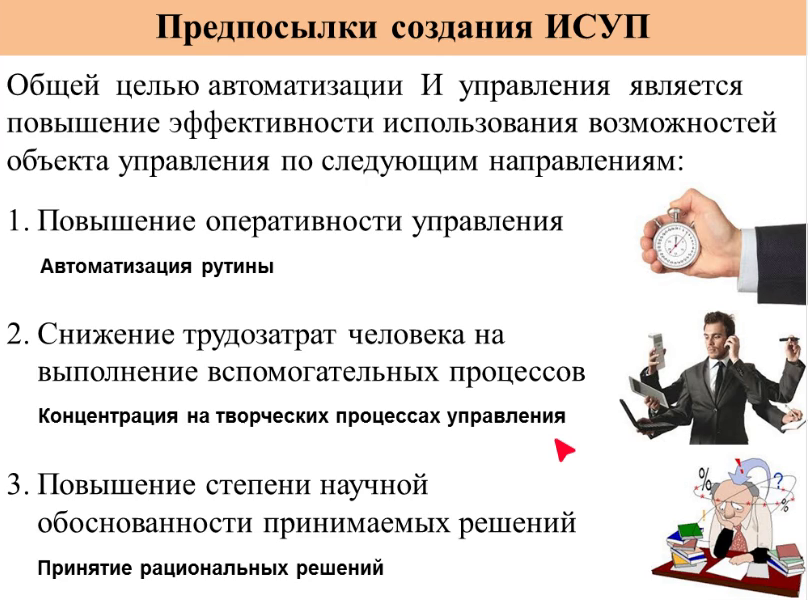
\includegraphics[width=\linewidth]{\picPath/tmpl_matching_inp.png}
    \caption{Исходное изображение}
  \end{subfigure}
  \begin{subfigure}[b]{0.4\linewidth}
    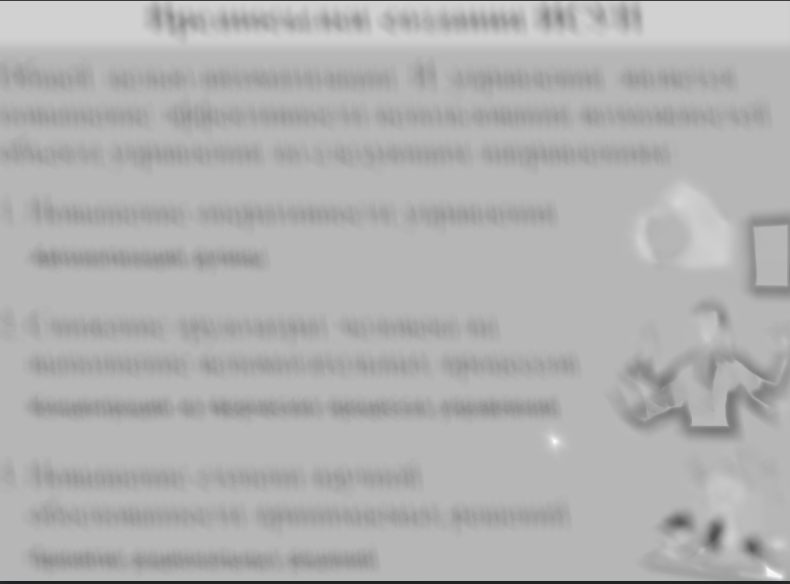
\includegraphics[width=\linewidth]{\picPath/match_template_mask.png}
    \caption{Результат применения свёртки}
  \end{subfigure}
  \begin{subfigure}[b]{0.4\linewidth}
    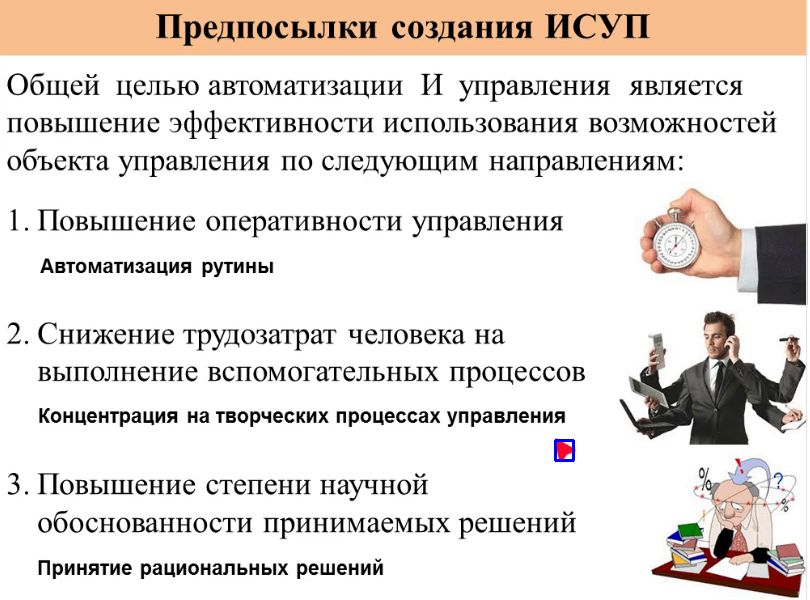
\includegraphics[width=\linewidth]{\picPath/templ_matching_result.png}
    \caption{На исходном изображении локализован курсор}
  \end{subfigure}
  \caption{пример работы алгоритма поиска изображения по шаблону}
  \label{fig:templateMatching}
\end{figure}

Достоинство метода  - высокая точность нахождения фрагментов изображений.

Недостатки - высокая точность достигается только в случае, когда фрагмент того же размера и не повернут относительно шаблона. 
	
	Существуют также методы, инвариантные относительно размера и положения искомого элемента и перспективы. Их называются \textit{методами совпадения по признакам}. Суть методов совпадения по признакам заключается в том, что из шаблонного изображения выделяются некоторые характерные признаки. После, в большом изображении находится объекты, схожие по признакам с шаблоном. Этот  класс методов избыточен для решаемой в этой работе задече.
	
\chapter{Пеобразование Фурье}
Для анализа аналоговых и цифровых сигналов зачастую используются дискретные преобразования, переводящие сигнал из одного базиса в другой. Многие операции над сигналом значительно упрощаются в частотном базисе, позволяя ускорить алгоритмы машинного зрения. Рассмотренные ниже преобразования представляют сигнал в виде суперпозиции частот. 
\section{Непрерывное преобразование Фурье}


Непрерывное преобразование Фурье имеет вид: 

Прямое:
\begin{equation}
F(s) 
\equiv
\mathcal{F}\{f(x)\}(s)
\equiv
{\int\limits_{-\infty}^{\infty}f(x)\,e^{-2\pi i s x}\,dx~}
\end{equation}

Обратное: 
\begin{equation}
f(x) 
\equiv
\mathcal{F}^{-1}\{F(s)\}(x)
\equiv
{\int\limits_{-\infty}^{\infty}F(s)\,e^{2\pi i s x}\,ds~}
\end{equation}

Где $f(x)$ - непрерывная функция - сигнал вещественной переменной,
$F(x)$ - непрерывная функция комплексной переменной - Фурье образ $f(x)$ \cite{Gonzalez}. 

Сверткой называют интегральное преобразование вида:
\begin{equation}
(f*g)(x)
=
{\int\limits_{-\infty}^{\infty} f(y)\,g(x-y)\,dy~} 
=
{\int\limits_{-\infty}^{\infty} f(x-y)\,g(y)\,dy~}  
\end{equation}

Корреляцией двух функций называют преобразование вида:
\begin{equation}
(f \star g)(x) 
= 
{\int\limits_{-\infty}^{\infty} f(y)\,g(x+y)\,dy~} 
= 
{\int\limits_{-\infty}^{\infty} f(x+y)\,g(y)\,dy~}  
\end{equation}

Доказана теорема свертки 
\begin{equation}
{(f*g)(x)}
\equiv
\mathcal{F}^{-1} \{
\mathcal{F}(f) \cdot \mathcal{F}(g) 
\}
\label{correlation_theorem}
\end{equation}

Аналогично теореме о свертке, существует теорема о корреляция 
\begin{equation}
{(f \star g)(x)} 
\equiv
\mathcal{F}^{-1} \{
\mathcal{F}^*(f) \cdot \mathcal{F}(g) 
\}
\end{equation}

Где операция \hspace{3pt} $\cdot$ \hspace{3pt} $-$ скалярное произведение, а $\mathcal{F}^*(f)$ - комплексно сопряженный образ Фурье функции $f$ .

\section{Дискретное преобразование Фурье}
Известно, что компьютер оперирует исключительно конечным набором цифровых данных и не может напрямую обрабатывать аналоговые сигналы. Поэтому первым этапом компьютерной обработки любого сигнала является его дискретизация т.е представление в виде конечной последовательности точек аргумент- значение.
Рассмотрим дельта функцию 

\begin{equation*}
\delta(t)=
\begin{cases}
\infty & t = 0 \\
0	 & t \neq 0
\end{cases}
\quad , \quad
{\int\limits_{-\infty}^{\infty}\delta(t)\,dt~}
=
1
\end{equation*}

Имеющую свойства

\begin{gather*}
{\int\limits_{-\infty}^{\infty}f(t)\delta(t)\,dt~}
=
f(0)
\\
{\int\limits_{-\infty}^{\infty}f(t)\delta(t-t_{0})\,dt~}
=
f(t_{0})
\end{gather*}

Если функция $f(t)$ - дискретная, то рассматривается дискретная дельта функция 
\begin{equation}
\delta(t)=
\begin{cases}
1 & t = 0 \\
0	 & t \neq 0
\end{cases}
\end{equation}

Тогда
\begin{gather}
\sum_{t = - \infty}^{\infty} \delta(t) 
=
1
\\
\sum_{t = - \infty}^{\infty} f(t) 
\delta(t - t_{0}) 
=
f(t_{0})
\end{gather} 

Рассматривая функцию, называемую серия импульсов (в англоязычной литературе train of impulses)
\begin{equation}
s_{\varDelta T}(t) 
=
\sum_{k=-\infty}^{\infty}
\delta(t - k\varDelta T)
\end{equation}

И её образ Фурье 
\begin{equation}
S(\mu) = \mathcal{F}
\{ s_{\varDelta T}(t)  \}
=
\frac{1}{\varDelta T}
\sum_{n = - \infty}^{\infty}
\delta(
\mu - \frac{n}{\varDelta T}
)
\end{equation}

Можем построить математическую модель дискретизации
функции $f(t)$ с соотвeтвующим Фурье образом $F(s) = \mathcal{F}\{f\}(s)$  следующим образом
\begin{equation}
\tilde{f}(t) = 
f(t)s_{\varDelta T}(t)
=
\sum_{n = -\infty}^{\infty}
f(t)
\delta(t - n\varDelta T)
\end{equation}

Тогда рассматривая образ Фурье дискретной функции, используя теорему свертки \ref{correlation_theorem},  можно получить \cite{Gonzalez}
\begin{equation}
\tilde{F}(\mu) = 
\frac{1}{\varDelta T}
\sum_{n = - \infty}^{\infty}
F(
\mu - \frac{n}{\varDelta T}
)
\label{Furier_sampling_result}
\end{equation}

Пусть значения $F(\mu)$  ограничены $[-\mu_{max},\mu_{max} ] $ т.е. частоты $f(t)$ ограничены  (в англоязычной литературе band limited functions) и 
пусть частота при дискретизации удовлетворяет неравенству:
\begin{equation}
\frac{1}{\varDelta T} 
>
2\mu_{max}
\end{equation}

Из \ref{Furier_sampling_result} и предыдущего неравенства очевидно, что $\tilde{F}(\mu)$ и $F(\mu)$ связаны соотношением
\begin{equation}
F(\mu)
=
H(\mu)
\tilde{F}(\mu)
\end{equation}

Где 
\begin{equation}
H(\mu)
=
\begin{cases}
\varDelta T & 
\mu \in [-\mu_{max},\mu_{max}] \\
0 & иначе
\end{cases}
\end{equation}

Обратное преобразование $H(\mu)$ имеет вид
\begin{gather*}
h(t)
=
\mathcal{F}^{-1}\{H(\mu)\}(t)
=
\int\limits_{-\infty}^{\infty}
H(\mu)
e^{2\pi i \mu t }
d\mu~
=
\int\limits_{-\mu_{max}}^{\mu_{max}}
\varDelta T
e^{2\pi i \mu t }
d\mu~
=
\\
=
\frac{\varDelta T}
{i 2 \pi t} 
\left[
e^{	2\pi i \mu t }
\right]_{-\mu_{max}}^{\mu_{max}}
=
2\varDelta T \mu_{max}
\frac{sin(2\pi t \mu_{max}) }{(2\pi t \mu_{max})}
=
2\varDelta T \mu_{max}
sinc(2t\mu_{max})
\end{gather*}

Отсюда следует вывод:  допуская, что частота $f(t)$ ограничена по модулю значением $\mu_{max}$, зная $\tilde{f}(t)$, которая получена сэмплированием из $f(t)$ c частотой не меньше, чем $2 \mu_{max}$,  можем приблизить $f(t)$ с любой точностью. 

Вычислить $f(t)$ через $\tilde{f}(t)$ можно следующим образом:
\begin{gather*}
f(t)
=
\mathcal{F}^{-1}
\{ F(\mu) \}
\\
=
\mathcal{F}^{-1}
\{
H(\mu)\tilde{F}(\mu)
\}
\\
=
h(t)*\tilde{f}(t)
\end{gather*}

или 
\begin{equation}
f(t) 
=
2  \mu_{max} \varDelta T
\sum_{ n = - \infty}^{\infty}
f(n \varDelta T ) 
sinc[ 2  \mu_{max}  (t - n \varDelta T) 	]
\end{equation}

Если же $ \varDelta T = \frac{1}{2 \mu_{max}} $ :
\begin{equation}
f(t) 
=
\sum_{ n = - \infty}^{\infty}
f(n \varDelta T ) 
sinc[ (t - n \varDelta T) / \varDelta T	]  
\end{equation}

Данный вывод называется \textit{теоремой Котельникова или сэмплирования.} 
Этот подход широко используется в обработке изображений и звука. Например зная, что человек слышит звуки частоты от 16 до 20 000 Гц можно без какой-либо потери информации для человеческого слуха записывать звуки с частотой дискретизации 44100 Гц.

\section{Двумерное преобразование Фурье}
Все теоремы и свойства, рассмотренные выше, распространяются на случай функции $n$ переменных. Рассмотрим двумерный случай. Для непрерывного сигнала $f(x,y)$ преобразование Фурье имеет вид
\begin{gather}
\label{FFT_2d}
F(\mu,\nu)
=
\int\limits_{-\infty}^{\infty}
\int\limits_{-\infty}^{\infty}
f(t,z) \,
e^{-i 2 \pi( \mu t + \nu z)}
dz dt~
\\
\label{IFFT_2d}
f(t,z)
=
\int\limits_{-\infty}^{\infty}
\int\limits_{-\infty}^{\infty}
F(\mu,\nu) \,
e^{i 2 \pi( \mu t + \nu z)}
d\mu d\nu~
\end{gather}

Последовательность импульсов в двумерном случае будет выглядеть так:
\begin{equation}
S_{ \varDelta T \varDelta Z }
(t,z)
=
\sum_
{ m = - \infty}^{\infty}
\sum_
{ n = - \infty}^{\infty}
\delta(
t - m \varDelta T,
z - n \varDelta Z
)
\end{equation}

Предполагая, что частоты функции $f(x,y)$ ограничены в $
[- \mu_{max},\mu_{max}] 
\times
[- \nu_{max},\nu_{max}] 
$
для “сжатия функции без потерь” достаточно взять
\begin{gather}
\varDelta T 
<
\frac{1}{2 \mu_{max}}
\\
\varDelta Z 
<
\frac{1}{2 \nu_{max}}
\label{Kotelnicov_imparity}
\end{gather}

Цифровые изображения хранятся как набор пикселей. Пусть дано изображение $M\times N$. Чтобы представить его в пространственном базисе, можно, например, положить, что один пиксель есть единица измерения пространства. Тогда изображение моделируется формулой вида
\begin{equation}
\tilde{f}(t,z) 
=
f(t,z)
S_{ \varDelta T \varDelta Z }
=
\sum_
{ m =  0}^{M-1}
\sum_
{ n =  0}^{N-1}
f(t,z)\delta(
t - m \varDelta T,
z - n \varDelta Z
)
\label{sample_2d}
\end{equation}

Где $\varDelta t = \varDelta z = 1$. Тогда соответствующие частоты будут изменяться в 
 пределах $[-\frac{1}{2},
\frac{1}{2}]
\times
[-\frac{1}{2},
\frac{1}{2}]$ согласно \refeq{Kotelnicov_imparity}.Таким частотам соответствуют периоды в пикселях: $[...,-3,-2] \cup [2,3,...]$.
Подставляя выражение \refeq{sample_2d} в прямое преобразование Фурье \refeq{FFT_2d}, получим
\begin{equation}
F(\mu,\nu)
=
\sum_
{ x =  0}^{M-1}
\sum_
{ y =  0}^{N-1}
f(x,y)
e^{
-i2\pi(\mu x / M +
 \nu y / N )
}
\label{DFFT_2d}
\end{equation}

Подставляя \refeq{DFFT_2d} в обратное преобразование \refeq{IFFT_2d}, получим
\begin{equation}
F(x,y)
=
\sum_
{ \mu =  0}^{M-1}
\sum_
{ \nu =  0}^{N-1}
f(\mu,\nu)
e^{
 i2\pi(\mu x / M +
 \nu y / N )
 \label{DIFFT_2d}
}
\end{equation}

откуда видно, что для восстановления исходного изображения достаточно всего $M\times N$ значений образа Фурье в точках $[0,M-1] \times [0,N-1]$.
 Формулы \refeq{DFFT_2d} и \refeq{DIFFT_2d} называется прямым и обратным двумерным конечным дискретными преобразованием Фурье соответсвенно.

\chapter{ Приложения преобразования Фурье }
\section{Сжатие и увеличение изображений}
Так как все Фурье образы - периодические функции как суперпозиция синусов и косинусов, то образ Фурье можно вычислить для любой точки пространства. Тогда в выражении  \refeq{DFFT_2d} 
 в суммах можем использовать любые пределы.
Тогда, чтобы изменить размер изображения с $M\times N$ на произвольный $m\times n$, $m >0$, $n > 0$, достаточно просто поменять пределы в формуле \refeq{DFFT_2d}.

\section{Свертка изображений}

Как было показано выше (\refeq{correlation_theorem}), свертка двух функций в пространственном базисе эквивалентна по элементному произведению в частотном. В Частности, в случае изображений: вместо очевидного метода свертки, когда окно скользит по изображению и на каждой итерации вычисляется значение пикселя, можно перевести изображение и ядро фильтра в частотный базис посредством прямого преобразования Фурье, выполнить скалярное произведение двух образов и последним шагом преобразовать произведения образов в пространственный базис с помощью обратного преобразования Фурье. 

Очевидный метод требует $MNmn$ операций для свертки изображения размера $M\times N$ с ядром размерности $m\times n$. Свертка же посредством преобразования Фурье, вместе со всеми преобразованиями требует $2MNlog_2(MN)$ Операций, что в случае большой размерности ядра значительно уменьшает число вычислений. 

\section{Алгоритм быстрой  кросс кореляции}
Данный алгоритм  - разновидность поиска по шаблону \cite{Cross-Correlation}. Главное его отличие в том, что для метрики представляет из себя корелляцию. Благодаря этому для нахождения шаблона в изображении можно использовать преобразование Фурье и значительно уменьшить количество вычислений. 
Рассмотрим метрику вида:

\begin{equation}
\gamma(u,v)
=
\frac{
\sum_{x,y}
[f(x,y) - \overline{f}_{u,v}]
[t(x-u,y-v)-t]
}
{
\sqrt{
\sum_{x,y}
[f(x,y) - \overline{f}_{u,v}]^2
\sum_{x,y}
[t(x-u,y-v)-t]^2
}
} 
\end{equation}

где
\begin{gather*}
t'(x,y)
\equiv
t(x,y) - \overline{t}
\\
f'(x,y)
\equiv
f(x,y) - \overline{f}_{u,v}
\end{gather*}

Тогда можем вычислить числитель как
\begin{equation}
\gamma_{num}(u,v)
=
\mathcal{F}^{-1}
\{
\mathcal{F}(f')
\mathcal{F}^*(t')
\}
\end{equation}

В знаменателе второе слагаемое всегда константа. Первое слагаемое можно вычислить, используя только $3M^2$   вместо $3N^2(M-N+1)$ операций, если использовать подход бегущей суммы (интегрирование изображений). 
Сравнивая методы поиска шаблона можно заметить, что методы быстрой кросс корелляции рабоатет на порядок быстрее алгоритмов, не использующих преобразование Фурье. 

Данный алгоритм был разработан специально для фильма “Форест Гамп”(1994) и использовался в большом количестве других проектов. Во время производства фильма было необходимо вырезать и заменить некоторые части изображения из видеопотока. Шаблон вручную выделялся, а после автоматически отслеживался на протяжении всей сцены посредством алгоритма быстрой кросс-кореляции. Найденные координаты использовались для дальнейших спецэффектов.

\begin{table}[H]
\caption{
сравнения времени работы стандартного и ускоренного алгоритма кросс корреляции. Тест предполагал координаты шаблона в кадрах из фильма “Форест Гамп”
}
\begin{tabularx}{\textwidth}{|X|X|X|X|}
\hline
Размер шаблона
&
Кол-во кадров
&
Время работы стандартного алгоритма
&
Время работы ускоренного алгоритма
\\
\hline
$168 \times 86$ & 896 & 15 часов & 1.7 часа 
\\
\hline
$	 115\times 200 \newline 150 \times 150 $
 & 490  &14.4 часа & 57 минут 
\\
\hline
\end{tabularx}
\end{table}

\chapter{Методы локализации текста на изображении}
Проблема распознавания текстовых изображений появилась давно \cite{JDAR_survey}. Системы распознавания текста из изображения (Optical Character Recognition) нашли своё применеия во многих отраслях жизни:

\begin{itemize}
\item чтение регистрационных знаков транспортных средсв;
\item определение и чтение дорожных знаков;

\item мобильное приложение для слабовидящих, распознающее и проговаривающее текст из изображения;

\item ввод информации;

\item оцифровка или архивация документов, видеопотока с камеры наблюдения и так далее.

\end{itemize}

На сегодняшний день алгоритмы локализации текста развиты достаточно хорошо. Тем не менее, они не могут дать абсолютно точный результат так как входные данные могут быть подвержены искажениям. Основные из них

\begin{itemize}

\item низкое разрешение; 

\item неравномерное освещение;

\item георметрические искажения;

\item дисторсия;

\item сложный фон;

\item шумы итд.

\end{itemize}

Задача распознавания текста не может быть поставленна точно: в некоторых ситуациях текст невозможно распознать физически, буквы не могут быть распознанны однозначно. Этот факт не уменьшает ответсвенности, возложенной на разработчика алгоритма распознавания образов.

Первый   этап большинства алгоритмов распознавания текста - его локализация. Главное отличие текста от фона и изображенй - высокий контарст. Кроме того, текст чаще всего имеет некоторый шрифт, у которого есть постоянный размер. На изображениях  условно выделяют два вида текстовой информации: текст, который нанесен на объекты съемки то есть надписи на транспорте, вывески, реклама и текст, который нанесен поверх изображения или со скана документа и так далее. 

\section{Градиентные методы локализации текста}

Исходя из предположения о том, что символы имеют четкие границы, в отличие от другой информации, можно предположить, что пиксели, значения градиента в которых велико, являются границами изображенных символов. После того, как алгоритмы локализации текста, основанные на градиенте, найдут преполагаемые границы символов, эти границы группируются в текстовые блоки. Примеры реализации методов локализации текста, основанные на градиенте: 

Исследователи Лии и Канканхалли активно используют производную по оси $x$. Кувано дополнил предыдущие подходы: он предпологал текстовые блоки по оси $x$ и $y$ отдельно, а затем обединял результаты, оставляя только пересекающие области. Для вычисления компонент градиетна исследователи использовали ядра Собеля. 

Для группировки границ в области, разработчики используют морфологические оперции: дилатацию и наращивание \cite{Dup:coursache}. В некоторых работах на последнем этапе проводится верефикация результата предыдущих этапов.

Исследователи Вонг и Чен используют в своем алгоритме только производную по $x$. Они предполагают, что дисперсия производной в районе текстовых блоков будет выше, чем в других областях.  Применяя к результату вычисления пороговую бинаризацию, предполагаются границы текстовых блоков.  Кроме того, разные исследовали рассматривают разные каналы изоражений, применяя к каждому из них опрецию градиента.

Исследователь Ким в своём градиентном методе локализации номерных знаков кроме градиента изображения использует дисперсию градиента, плотность и дисперсию плотности границ символов. Этот метод основывается на предположении о том, что область номерного знака имеет большую дисперсию градиента, высокую плотность вычесленных градиентом границ и низкую дисперсию этой плотности.

Кроме того, некоторые исследователи используют для поиска областей текствовой информации нейронные сети. Исследователь Хуа на промежуточном этапе, после выполнения операции выделения границ,  вычисляет углы границ символов с помощью нейронных сете и впоследствии использует эту информацию для улучшения результата работы алгоритма. 

Семейство градиентых алгоритмов показывает высокую производительность, и при достаточно высоком качестве входных данных и малых искажениях работает точно.

\section{Алгоримы локализации текста, основанные на цветовых характеристиках изображения}

В основе семейства алгоритмов, основанных на цветовых характеристиках изображения, лежат алгоритмы сегментации изображений по цвету. Пердполагается, что текст имеет определенный цвет и яркость, что и отделяет его от фона.  После сегментации, также, как в градиентных методах, границы группируются и верефицируются. В общем случае, результат разделения изображения по цвету используется для выделения не только текста, но и любых объектов, схожих по цвету.

Например для сегментации, исследователь Миен использовал быстрый алгоритм сегментации по цвету, вычисляющий результат за один проход. Этот алгоритм можно описать следующим образом: сначала сравниваются пиксели, соседние в строке, а затем в столбце. На базе этой информации принимается решение, если ли в данной координате граница между цветом или нет.    

Другой популярный подход к цветовой сегментации изображений - квантование цветов. Квантование по сути - разбиение диапазона отсчетных значений сигнала на конечное число уровней и округление этих значений до одного из двух ближайших к ним уровней. Главное преимущество квантования $-$ высокая степень устойчивости к шумам. 

Использование несколько цветовых пространств $-$ распространенная практика при квантовании цветов. Исследователь Ли объединил результаты квантования из 27 различных цветовых индексов, рассматривая  отдельные биты значений цветов как каналы каналы. 

\section{Алгоритм локализации текста, основанный на текстуре}
Под текстурой подразумивают визуальные свойства каких-либо поверхностей или объектов.Предполагается, что текст имеет уникальную, отличную от фона текстуру. Текстураня информация может  Человек может отличить текст от фона даже тогда, когда язык текста ему неизвестен. Он отличает символы по текстуре. 

Описать текстуру изображения можно многими способами. Исследователь Шонг   предполагает, что области, содержашие текстовую информацию, содержат определенные высокие частоты, которые вычисляются при помощи дискретных преобразований. В своём алгоритме Шонг использовал дискретное косинус преобразование, которое по сути мало отличается от дискретного преобразования Фурье.  Ву для выделения структуры изображения сворачивал изображение с гаусианной и после классифицировал области алгоритмом k- среднего.

Для выделение текстурных особенностей широко используются нейронные сети. Исследователь Юнг  использовал многослойный перцептрон; нейронная сеть последовательно принимала на вход всевозможные малые области изображения и выносила вердикт: представлен символ или нет. Однако этот подход не типичен, чаще из изображения некоторым способом выделяются особенности, которые уже после классифицируются. Особенность изображения можно определит как некоторый объект, характерный данному изображению. Также, как и в других семействах алгоритмов, некоторые из представителей семейства текстурных алгоритмов рассматривают несколько каналов одного изображения, а затем объединяют результат. Нейронный классификатор обычно обучается на особенностях, выделенных из малых изображений.  

Сравнивая семейства методов локализации текста, авторы статьи \cite{JDAR_survey} пришли к выводу, что универсального алгоритма, который был бы лучше остальных по всем параметрам, нет.  Семейство текстурных алгоритмов имеет ряд преимуществ: устойчивые к шумам, способные на самообучение и имеющие некоторый запас уверенности в результате, они требуют на порядок больше вычислений, чем алгоритмы, основанные на разделении цвета и градиенте, которые имеют на порядок меньшую точность в сравнении с первым. 

Возможное решение этой задачи - композиция алгоритмов. На первом этапе области выделяются градиентным методом или алгоритмом, основанным на цветовой разнице. А для верификации результатов использовать один из трудозатратных алгоритмов, работающих с текстурой.   

Возможный подход к верификации быстрых алгоритмов локализации текста - попытка распознать полученный на предыдущем этапе текстовый блок.

\chapter{Программная реализация}
\section{Постановка задачи}
Тут постановка задачи
\section{Алгоритм сравнения изображений}
Одна из подзадач, поставленная в процессе разработки приложения, требует вычисления некоторой корреляции между парой изображений.  Алгоритм сравнения изображений получает на вход два экземнляра изображений и возвращает вещественное число из $[0,1]$, где $0$ - абсолютно разные изображения, $1$ - идентичные изображения.  В программной реализации алгоритма сравнения изображений используется описанные выше методы сравнения совпадения по шаблону.

Алгоритм сравнения изображений:

\begin{enumerate}%[label=\arabic*),ref=\arabic*]
\item на вход два изображения $x, y$;
\item если отношение max( ширина $x$, ширина $y$) / min ( ширина $x$, ширина $y$) > $1.5$ или max( длина $x$, длина $y$) / min ( длина $x$, длина $y$) > $1.5$ $-$ то изображения разные, вернуть $0$;
\item если  max ( кол-во не черных пикселей $x$,  кол-во не черных пикселей $y$ ) / min ( кол-во не черных пикселей $x$,  кол-во не черных пикселей $y$ ) > $10$ - изображения разные, вернуть $0$;
\item вычислить относительное положение: 

\begin{enumerate}%[label=\asbuk*),ref=\asbuk*]
\item длины сторон $x$ меньше, чем у $y$;
\item длины сторон $y$ меньше, чем у $x$;
\item одна из сторон $x$ больше, чем у $y$ и одна из сторон $y$ больше, чем у $x$;
\end{enumerate}

\item если а - $z = x$,$x = y$,$y = z$;
\item если в - добавить к элементу $y$ белую границу справа на ширину $x$, снизу на длину $x$
\item с помощью бинаризации вычислить маску для $x$
\item используя метод совпадения по шаблону с метрикой TM\_CCORR\_NORMED найти координаты наиболее похожего на $x$ окна в $y$
\item сравнить $x$ и полученное на предыдущем этапе окно из $y$ методом совпадения по шаблону с метрикой TM\_SQDIFF
\item полученная маска размером $1 \times 1$ есть квадрат разности между яркостями пислей изображения, вернуть $1$ - яркость пикселя маски / $255$.
\end{enumerate}

\section{Алгоритм поиска курсора}
Курсор можно определить как изображение, постоянно или почти постоянно находящееся в видео потоке, меняющее свое положение и не меняющее форму. Для поиска курсора и хранения изображения удобно использовать класс, реализующий, кроме поиска курсора, ряд вспомогательных функций

\begin{enumerate}
\item процедура очистки чёрно-белого изображения разности кадров от шумов;
\item процедура поиска границ областей в изображении.
\end{enumerate}

Кроме этого, используется процедура сдвига  видеопотока на величину shift и вычисления разности между текущим кадром и кадром, считанным до сдвига.
Разность вычисляется как абсолютная разность между векторами - значениями пикселей. Будем называть разность изображений нулевой, если результат будет отличаться от черного изображения только шумом.

Алгоритм поиска курсора в видеопотоке:

\begin{enumerate}
\item на вход дан видеопоток;
\item вычислить  разность между кадрами;
\item сохранить кадр до свига видеопотока как текущий слайд;
\item сгенерировать маску курсора для текущего слайда;
\item пока маска не черная и количество не черных элементов разности меньше, чем 3 площади изображения курсора:
\begin{enumerate}
	\item вычислить разницу между кадрами;
	\item для текущего кадра вычислить маску курсора;
	\item вычислить маску для заполнения как маска кадра минус (маска кадра пересечение маска текущего слайда);
	\item вычислить новое значение маски слайда как пересечение маски слайда с текущей маской;
	\item из текущего слайда вырезать область по маске для заполнения и вставить в изображение текущего слайда;
\end{enumerate}
\item пока количество не черных элементов разности меньше, чем 3 площади изображения курсора вычислить разницу между кадрами;
\item сохранить текущий слайд в памяти.
\end{enumerate}

\section{Алгоритм генерации слайдов}
Алгоритм генерации слайдов вырезает слайды из видеопотока и пытается вырезать изображение курсора там, где это возможно.

Алгоритм генерации слайдов можно описать следующим образом:
\begin{enumerate}
\item на вход дано изображение слайда;
\item размыть изображение по Гаусу с ядром $3*3$;
\item бинаризовать изображение с порогом 180;
\item изменить изображение посредством морфологической операции эрозия с прямоугольным ядром 1 * предполагаемая минимальная высота буквы. 
\item отфильтровать изображение с ядром  
$\begin{bmatrix}
1 & 0 & -1 \\
2 & 0 & -2 \\
1 & 0 & -1
\end{bmatrix}$ для выделения левых границ объектов изображения
\item отфильтровать изображение с ядром 
$\begin{bmatrix}
-1 & 0 &  1 \\
-2 & 0 &  2 \\
-1 & 0 &  1
\end{bmatrix}$ для выделения правых границ объектов изображения;
\item наложить оба отфильтрованных изображения друг на друга;
\item посредством морфологических операций оставить только те прямоугольные области ширины 1, длина которых  входит в допустимый отрезок;
\item посредством морфологических операций объединить полученные области в предполагаемые текстовые блоки;
\item определить прямоугольные контуры вокруг предполагаемых текстовых блоков;
\item отфильтровать полученные контуры удалив те, которые по тем или иным причинам быть не могут контуром текстового блока.
\end{enumerate}

Алгоритм генерации слайдов на последнем этапе требует выполнения процедуры фильтрации контуров. В программной реализации используются несколько работающих последовательно фильтров. Первый из них удаляет все вложенные друг в друга контуры, и те, чья площадь была меньше допустимой. Второй фильтр пытается, кроме этого, отличить текстовый блок от других изображений основываясь на том факте, что текстовый блок можно разбить на строки, строки можно разбить на слова, а слова разбить на символы. Формы символов, в свою очередь, имеют определенные ограничения. В реализации для каждой строки вычисляется величина:
\begin{center}
\textit{
высота строки / среднее арифметическое ширины символа в строке.
}
\end{center}

После вычисляется медиана ряда полученных выше величин. Эта медиана $m$ проверяется неравенством
$1 \leq m \leq 3.5$. Если неравенство выполняется, то данный блок считается текстовым, иначе отбрасывается. 

 Для выделения строк текста для заданной области вычисляется вертикальная гистограмма как вектор, длина которого равна высоте выделенной области, а каждый элемент равен количеству не белых пикселей в соответствующей строке. Каждая непрерывная последовательность ненулевых элементов вектора определяет границей строки текста. Аналогичным способом в каждой найденной строке с помощью горизонтальной гистограммы вычисляются вхождения отдельных символов. Второй метод фильтрации мало устойчив к помехам и достаточно часто ошибается. Именно поэтому неравенство фильтра 2 проверяется не для каждой текстовой строки, а только для медианного случая. В силу того, что фильтр 2 работал некоректно, в конечной реализации алгоритма генерации слайдов он не использовался.

Последний фильтр использует для классификации библиотеку tesseract. Предполагаемый текстовый блок поступает на вход классификатора.  Если классификатор выдает сообщение “Empty page” или текст, который по некоторым критерием не может содержаться на изображении, то область удаляется из множества текстовых блоков. 

Библиотека tesseract достигает высокой точности в распознавании текстовых блоков, в то же время очень времязатратна: третий фильтр выполняется на порядок дольше двух предыдущих. Поэтому важно отфильтровать множество предполагаемых текстовых блоков как можно точнее до этапа распознавания слов.

\section{Работа библиотеки tesseract}

Tesseract - open-source OCR приложение, изначально разрабатываемое компанией HP в период 1984-1994 годов. В 2005 году HP выложила исходный код  в открытый доступ\cite{Smith:Tesseract}. 

Распознавание текста происходит в несколько шагов. На первом этапе изображение подвергается адаптивной бинаризации. Следующий шаг - анализ компонент связности. На этом этапе tesseract определяет контуры для каждой из компонент и полигонизирует их. Благодаря тому, что программа в дальнейшем рассматривает полигоны, а не изображение, вырезанное по контуру, она не зависит от цвета текста то есть черный текст на белом фоне распознается точно также, как белый текст на черном. 

После приложение пытается найти строки текста. Строки не обязательно должны быть строго горизонтальными, tesseract может выделить строку, повернутую на некоторый угол. После tesseract пытается разделить слова на символы. На первой итерации программа вычисляет предполагаемую ширину символа, просто делит полигоны вертикальными линиями и передает результат в статический классификатор. После каждой удачной попытки определить символ то есть когда вероятность, что данная область и некоторый ascii символ совпадают высока, область передается в адаптивный классификатор (adaptive classifier)  как набор обучающих данных. На следующих этапах классификации tesseract будет учитывать предыдущий опыт классификации, что сильно увеличивает точность.  В случае неудачи tesseract пытается сегментировать слова другими методами (non-fixed-
pitch). Сначала в полигонах определяются вогнутые вершины (concave  vertices). С помощью статического классификатора, как и на предыдущем этапе, определяются пары найденный вершин, проведя прямую через которые вероятнее всего отдельный полигон будет поделен на символы. 


Если после этого некоторые слова так и не удалось распознать, tesseract предполагает, что символы на изображении составлены не из одного полигона, а из нескольких т.е. символы при адаптивной бинаризации разбились на несколько отдельных компонент связности. На этом этапе полигоны проходят через так называемый ассоциатор (associator), который основан на алгоритме направленного поиска A*. Ассоциатор ищет такую комбинацию изначальных компонент связности, что она уверенно определяется классификатором как символ. Авторы tesseract соглашаются с тем, что процесс “Разбить изображение на минимальные компоненты связности, а затем соединять их” может быть не оптимальным, но аргументируют выбор такой последовательности тем, что входные данные ассоциатора упрощаются, благодаря чему поиск может вестись быстрее. Когда данный алгоритм был впервые реализован в tesseract в 1989 году, точность распознавания разбитых на несколько областей символов программы была намного больше, чем у конкурентов.

После того, как слова распознаны, tesseract проводит лингвистический анализ: для каждого слова в словаре находится наиболее похожая аналогия. Аналогичное слово может отличатся от распознанного не только символами, но и их количеством.

Классификация символов проходит в два этапа. Из входа извлекаются особенности или фичи (features), которые сравниваются с особенностями символов, выделенных в процессе обучения. Классификатор имеет два вида особенностей: трехмерный вектора, содержащие координаты и углы, и четырехмерные вектора, которые хранят кроме углов и координат еще и длину. На первом этапе строится список символов, на которые входной символ может быть похож, причем производится сравнения только трехмерных особенностей, что гораздо менее трудозатратно и позволяет  на раннем этапе классифицировать вход как не символ. На втором этапе каждый из избранных символов представляется как логическая сумма произведений четырехмерных фич. Вычисляется расстояние между входом и каждым символом, на основе которого строится окончательное решение. Благодаря представлению, при вычислении расстояний tesseract распоряжается информацией о расстоянии между каждой особенностью в отдельности, а не глобальным расстоянием между контурами, что увеличивает точность классификации .  Авторы tesseract опытном путем выявили, что при сравнении четырехмерных особенностей относительно короткие особенности резко отличаются у разбитых на части и целых символов. Поэтому для увеличения точности tesseract не использует относительно короткие особенности. 

После более чем десятилетнего перерыва, tesseract отстает от современных коммерческих OCR приложений в точности распознавания текстов. Тем не менее, tesseract остается популярным среди разработчиков благодаря открытому исходному коду, достаточно высокой точности распознавания и активной поддержкой сообщества (в том числе разработчиками google). 
\chapter{Программная реализация}

\newpage
\addcontentsline{toc}{chapter}{Заключение}
\begin{center}
\bfseries ЗАКЛЮЧЕНИЕ
\end{center}

\newpage
%список литературы
\addcontentsline{toc}{chapter}{Список использованных источников}
\begin{thebibliography}{0}

\bibitem{Smith:Tesseract}           	
Smith R. An Overview of the Tesseract OCR Engine \urlTitle
\url{https://static.googleusercontent.com/media/research.google.com/ru//pubs/archive/33418.pdf} (12.03.2019)
%\bibitem {Digital_proc}Эмануил Айфичер Цифровая обработка сигналов

\bibitem {Gonzalez}
  Gonzalez R.C.,  Woods R.E. Processing digital Image 4 global edition $-$ M: Pearson, 2017. $-$ 993с. 

\bibitem {Cross-Correlation} 
Lewis J. P. Fast Normalized Cross-Correlation 
\urlTitle \url{http://scribblethink.org/Work/nvisionInterface/nip.html} (12.03.2019)

\bibitem {JDAR_survey}
Jian Liang, David Doermann, Huiping Li. Camera-based analysis of text and documents: a survey. \urlTitle \url{http://citeseerx.ist.psu.edu/viewdoc/download?doi=10.1.1.94.9236&rep=rep1&type=pdf} (12.03.2019)


\bibitem{Dup:coursache}
 Ляхов Д.А. Распознавание образров в условиях цветовой близости.  Кубан. гос. ун-т. – Краснодар, 2018. – 30 с.

\end{thebibliography}
\end{document} 